\graphicspath{{./}{./fig/}{./appendices/fig0/}}

\chapter{Mean field shaping and monitoring}\label{chap:appendices}


\section{Phase printing}

Controlling precisely the phase of a laser beam is a common but challenging task in optics. The most basic way to do it is by applying spatial filtering in the fourier plane of a lens.
The phase of the beam after a second collimating lens is then given by the covolution product of the beam phase and the mask inverse fourier transform. This method then show its limits when one wants to 
generate complex phase profile since its depend on the mask form. A way to overcome this problem is the use of Digital Micromirror Device (DMD) which is an array of micro-mirrors that can be individually controlled to reflect the light or not.
By putting this array in the fourier plan of a lens it is possible to create spatial filtering with arbitrary shapes. However, this method suffers from high losses and diffraction of the light on the individual mirrors that tend to 
add unwanted noise. This being said, DMD are very powerfull devices and allow to do a great amount of things at low cost. A wide range of possible methods are referenced in the great work \cite{wavefront_shapping}. 

\bigskip

\subsection{Spatial light modulator.} In this work, we use a Spatial Light Modulator (SLM) which is a liquid crystal display that can be used to modulate the phase of a laser beam. The principle is to apply a voltage on each pixel of the SLM to change the orientation of the liquid crystal molecules. 
The phase shift is then given by the difference of the optical path of light going through the different pixels as shown in \autoref{fig:SLM}. 

\begin{figure}
    \centering
    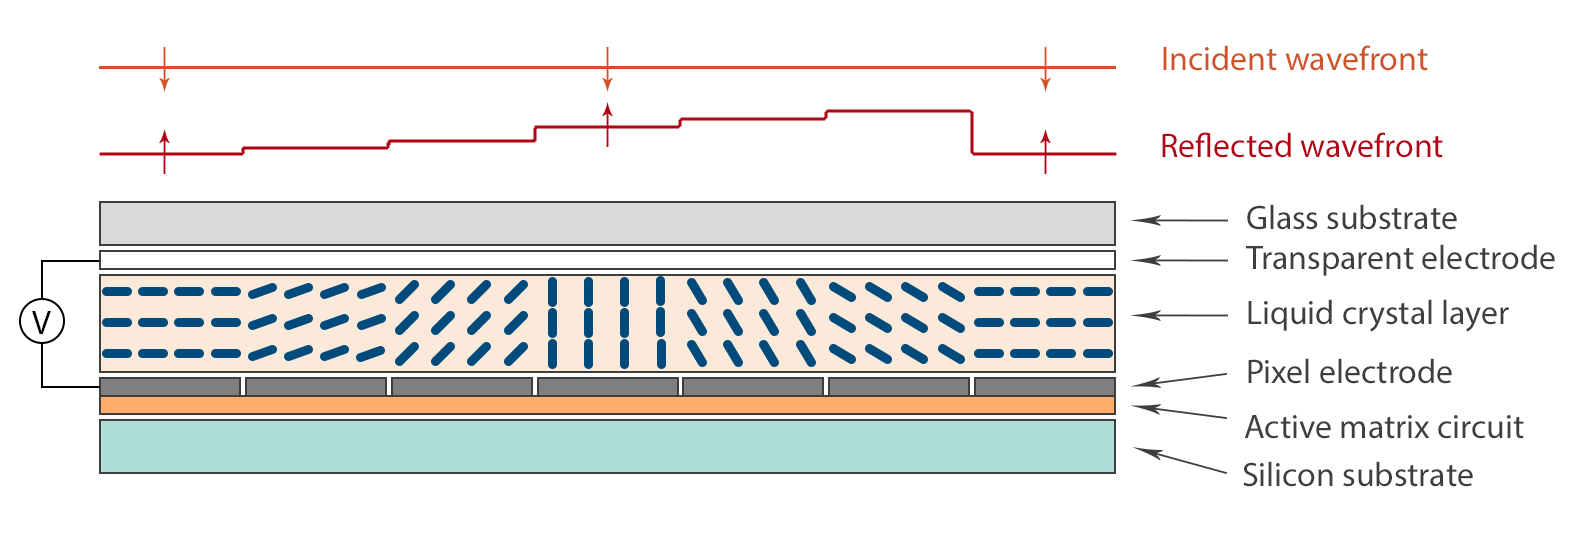
\includegraphics[width=1\textwidth]{appendices/fig0/SLMprinciple.png}
    \caption{Principle of a Spatial Light Modulator.}
    \label{fig:SLM}
\end{figure}

\noindent By shinning a flat phase collimated beam on the SLM which displays the target phase profile the beam gets reflected carrying the desired wavefront.
However the efficiency of the SLM is not perfect and whenever light is shone on it, some photons migth not see it and not be phase modulated. To overcome this difficulty,
we first write a blazed phase grating on the SLM screen on top of which the wanted profile is set. All the photons that did interact with the liquid crystals are then mostly diffracted on the first order of the grating. Doing so,
an efficiency of 60-70\% can be reached. This contrast with the usual 80\% usually claimed on manufacturer datasheets that actually correspond to the efficiency in all orders. A typical phase profile encoded on the SLM is shown
in \autoref{fig:SLM_profile}. A gray value of zero correspond to no shift while 255 corresponds to $2\pi$. The gray map corresponding to the target phase profile has been unwrapped for the sake 
of clarity and is shown in \autoref{fig:SLM_profile} c). The final gray map displayed on the SLM screen in represented in \autoref{fig:SLM_profile} e). 

\begin{figure}
    \centering
    \hspace{-1.4cm}
    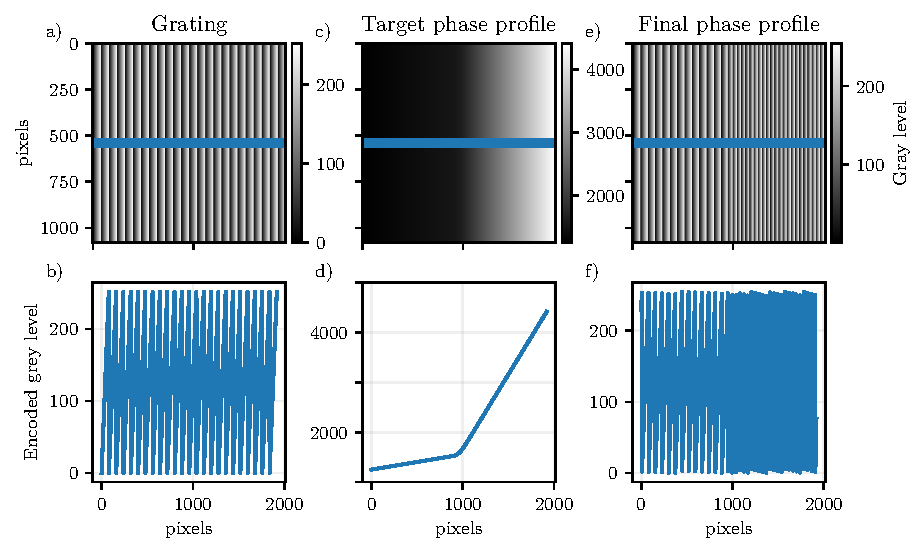
\includegraphics[width=1.1\textwidth]{appendices/fig0/slm_typical.pdf}
    \caption{Typical profile encoded on the SLM to generate the target velocity profile. a) Gray map of a phase blazed grating encoded on the SLM screen and b) corresponding cut in the 
    $x$ direction. c) Unwrapped grey map of the target phase profile and d) corresponding cut in the $x$ direction. e) Final gray map encoded on the SLM screen and f) corresponding cut in the $x$ direction. This map is the sum 
    of the blazed grating and the target phase profile modulus 255.} 
    \label{fig:SLM_profile}
\end{figure}

To imprint precisely the resulting wavefront in the cavity plane two $2f-2f$ optical telescopes are used in series to image the SLM screen with an overall demagnification of 1/130 while avoiding short focal lenght that would introduce optical aberrations.
An adjustable slit is placed in the fourier plane of the first telescope to filter out the unwanted diffracted orders.

\subsection{Phase measurement}
\label{sec:phase_measurement}

\subsection{Off axis inteferometry}
The principle is the following :
the beam whose phase is to be measured is recombined on a CCD camera with a flat phase reference beam. An angle is volontary introduced between the two beam to create an interference pattern on the camera plane. The phase difference between 
the two beams is then encoded in the size of the fringes and can be recovered by performing a fourier transform on the interferogram and demodulate the signal around the satellite peak created by the angle between the two beams \cite{liebling_complex-wave_2004}.

\subsection{Controlling the local intensity}

\label{sec:local_intensity}